\documentclass[a4paper,12pt,openany,oneside,headings=optiontohead]{scrbook} % kodovanie diakritiky je utf-8
\usepackage[utf8]{inputenc}
\usepackage[slovak]{babel}
\usepackage{a4wide,color}
% \usepackage[includehead, includefoot, top=2.5cm, bottom=2.5cm, left=3.5cm, right=2cm]{geometry}
\usepackage[includehead, includefoot, top=2.5cm, bottom=2.5cm, left=2.75cm, right=2.75cm]{geometry}
% \usepackage[includehead, includefoot, top=0cm, bottom=0cm, left=0cm, right=0cm]{geometry}
\usepackage{lmodern}
\usepackage[T1]{fontenc}
\usepackage{fontenc}
\usepackage{amsfonts}
\usepackage{amssymb}
\usepackage{amsthm}
\usepackage{amsmath}
\usepackage{epsfig}
\usepackage{wrapfig}
\usepackage{graphicx}
\usepackage{caption}
\usepackage{subcaption}
\usepackage{url}
\usepackage[bookmarks]{hyperref}
\usepackage{fancyhdr}
\usepackage{indentfirst}
\usepackage{fancyvrb}
\usepackage{wasysym}
\usepackage{placeins}
\usepackage{multirow}
\usepackage{booktabs}

\ifpdf
  \usepackage{pdfpages}
\fi

\usepackage{listings}
\renewcommand\baselinestretch{1.3} % toto je riadkovanie jeden a pol, a nie {1.5}

%zdrojaky
\definecolor{dkgreen}{rgb}{0,0.6,0}
\definecolor{gray}{rgb}{0.5,0.5,0.5}
\definecolor{mauve}{rgb}{0.58,0,0.82}
\definecolor{ltyelloow}{rgb}{1,.96,0.93}

\lstset{ %
  language=python,                % the language of the code
  basicstyle=\footnotesize,           % the size of the fonts that are used for the code
  numbers=left,                   % where to put the line-numbers
  numberstyle=\tiny\color{gray},  % the style that is used for the line-numbers
  stepnumber=1,                   % the step between two line-numbers. If it's 1, each line
                                  % will be numbered
  numbersep=5pt,                  % how far the line-numbers are from the code
  backgroundcolor=\color{ltyelloow},      % choose the background color. You must add \usepackage{color}
  showspaces=false,               % show spaces adding particular underscores
  showstringspaces=false,         % underline spaces within strings
  showtabs=false,                 % show tabs within strings adding particular underscores
  frame=false,                   % adds a frame around the code %single
  rulecolor=\color{white},        % if not set, the frame-color may be changed on line-breaks within not-black text (e.g. commens (green here))
  tabsize=2,                      % sets default tabsize to 2 spaces
  captionpos=b,                   % sets the caption-position to bottom
  breaklines=true,                % sets automatic line breaking
  breakatwhitespace=false,        % sets if automatic breaks should only happen at whitespace
  title=\lstname,                   % show the filename of files included with \lstinputlisting;
                                  % also try caption instead of title
  keywordstyle=\color{blue},          % keyword style
  commentstyle=\color{dkgreen},       % comment style
  stringstyle=\color{mauve},         % string literal style
  escapeinside={\%*}{*)},            % if you want to add a comment within your code
  morekeywords={*,...},               % if you want to add more keywords to the set
  literate={č}{{\v{c}}}1
           {í}{{\'i}}1
}

%makra
\newtheorem{vt}{Veta}[section]
\newtheorem{lema}[vt]{Lema}
\theoremstyle{definition}
\newtheorem{df}[vt]{Definícia}

% pekne pokope definujeme potrebne udaje
\def\mftitle{Zarovnávanie sekvencií s~použitím metód klasifikácie}
\def\mftitlefirst{Zarovnávanie sekvencií s~použitím metód klasifikácie}
\def\mftitlesecond{}
\def\mfthesistype{Diplomová práca}
\def\mfauthor{Bc. Michal Hozza}
\def\mfadvisor{Mgr. Tomáš Vinař, PhD.}
\def\mfconsultant{Mgr. Michal Nánási}
\def\mfdate{2014}
\def\mfplacedate{Bratislava, \mfdate}
\def\mfuniversity{Univerzita Komenského, Bratislava}
\def\mffakulta{Fakulta Matematiky, Fyziky a Informatiky}
% \ifx\pdfoutput\undefined\relax\else\pdfinfo{ /Title (\mftitle) /Author (\mfauthor) /Creator (PDFLaTeX) } \fi

\def\todo{{\color{red} ToDo: }}
\def\method#1{{\tt #1}}

\ifpdf
  \pdfinfo{
    /Title (\mftitle)
    /Author (\mfauthor)
    /Creator (PDFLaTeX)
  }
\else
\fi

\begin{document}
\pagestyle{plain}
\frontmatter

\thispagestyle{empty}

\noindent
\begin{center}
\begin{minipage}{0.8\textwidth}
\centerline{\renewcommand\baselinestretch{1.3} \LARGE\sc\mfuniversity}
\centerline{\sc\mffakulta}
\end{minipage}
\end{center}

\vfill
\begin{center}
\begin{minipage}{1\textwidth}
\begin{center}
\linespread{1}\LARGE\sc\mftitle
\end{center}
\smallskip
\centerline{\mfthesistype}
\end{minipage}
\end{center}
\vfill
{\bf
\begin{minipage}{0.4\textwidth}
\begin{flushleft} \large
~\mfdate
\end{flushleft}
\end{minipage}
\begin{minipage}{0.59\textwidth}
\begin{flushright} \large
\mfauthor
\end{flushright}
\end{minipage}
}
\eject % EOP i

\thispagestyle{empty}

\noindent
\begin{center}
\begin{minipage}{0.8\textwidth}
\centerline{\LARGE\sc\mfuniversity}
\centerline{\sc\mffakulta}
\end{minipage}
\end{center}

\vfill
\begin{center}
\begin{minipage}{1\textwidth}
\bigskip\bigskip
\begin{center}
\linespread{1}\LARGE\sc\mftitle
\end{center}
\smallskip
\centerline{\mfthesistype}
\bigskip
\bigskip
\bigskip\bigskip
\end{minipage}
\end{center}
\vfill
\begin{minipage}{0.8\textwidth}
\begin{tabular}{l l}
Študijný program:& Informatika \\
Študijný odbor:& 2508 Informatika \\
Školiace pracovisko:& Katedra Informatiky\\
Školiteľ:&   \mfadvisor \\
Konzultant:&   \mfconsultant \\
\end{tabular}
\end{minipage}
\vfill
{\bf
\begin{minipage}{0.4\textwidth}
\begin{flushleft} \large
~\mfplacedate
\end{flushleft}
\end{minipage}
\begin{minipage}{0.59\textwidth}
\begin{flushright} \large
\mfauthor
\end{flushright}
\end{minipage}
}
\eject % EOP iii

%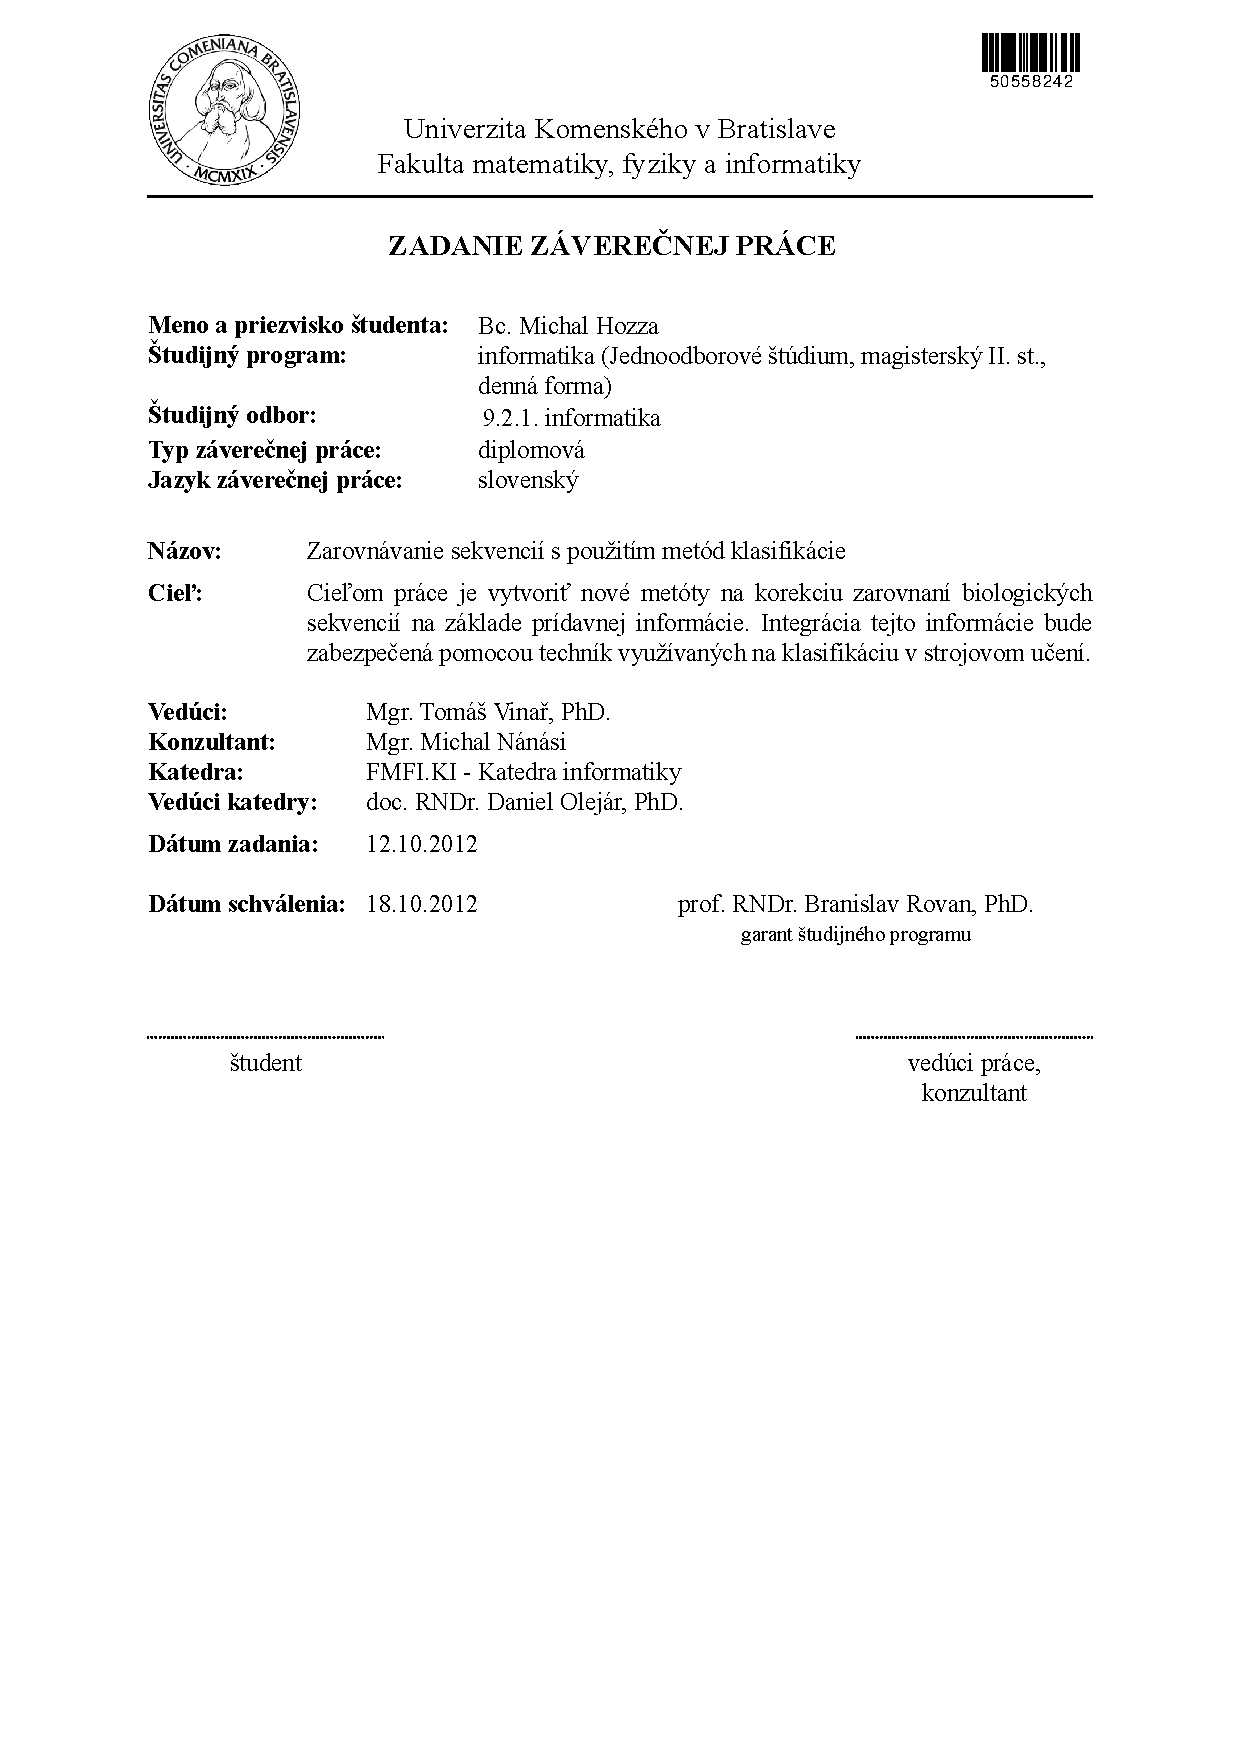
\includepdf{zadanie.pdf}

{~}\vspace{12cm}

\noindent
\begin{minipage}{0.25\textwidth}~\end{minipage}
\begin{center}
\begin{minipage}{1\textwidth}
%Ďakujem vedúcemu bakalárskej práce Marekovi Nagyovi za cenné rady
%a pripomienky, bez ktorých by táto práca asi nevznikla, priateľke, blízkym priateľom a rodine za morálnu podporu.
Poďakovanie...
\end{minipage}
\end{center}
\hfill\mfauthor
\vfill\eject % EOP v
% ~\vfill\eject % EOP vi % zadna strana prehlasenia je prazdna


\noindent
%\begin{minipage}{0.25\textwidth}~\end{minipage}
\begin{center}
\begin{minipage}{1\textwidth}
\centerline{\large Abstrakt}
%\begin{center}
\input abstraktSK.tex
%\end{center}
\end{minipage}
\end{center}
\eject % EOP v
% ~\vfill\eject % EOP vi % zadna strana prehlasenia je prazdna

\noindent
%\begin{minipage}{0.25\textwidth}~\end{minipage}
\begin{center}
\begin{minipage}{1\textwidth}
\centerline{\large Abstract}
%\begin{center}
\input abstraktEN.tex
%\end{center}
\end{minipage}
\end{center}
\eject % EOP v
% ~\vfill\eject % EOP vi % zadna strana prehlasenia je prazdna

\tableofcontents
\listoffigures
\listoftables

\mainmatter
\pagestyle{fancyplain}
% \fancyhead[l]{}

\input kapitoly.tex

\backmatter

%\cleardoublepage
\phantomsection
\addcontentsline{toc}{chapter}{Literatúra}
\nocite{*}
\bibliographystyle{alpha}
\bibliography{literatura.bib}

\end{document}
